\UseRawInputEncoding
\documentclass[12pt,a4paper]{article}
\usepackage[utf8]{inputenc}
\usepackage[T1]{fontenc}
\usepackage[french]{babel}
\usepackage{geometry}
\usepackage{titlesec}
\usepackage[colorlinks=true, linkcolor=none]{hyperref}
\usepackage{listings}
\usepackage{xcolor}
\usepackage{float}
\usepackage{graphicx} 
\usepackage[most]{tcolorbox}
\geometry{margin=2.5cm}




\lstset{
  basicstyle=\ttfamily\small,
  backgroundcolor=\color{gray!10},
  frame=single,
  breaklines=true
  showspaces=false
  inputencoding=utf8,
  extendedchars=true,
  literate=
    {é}{{\'e}}1
    {è}{{\`e}}1
    {ê}{{\^e}}1
    {à}{{\`a}}1
    {ù}{{\`u}}1
    {â}{{\^a}}1
    {î}{{\^i}}1
    {ç}{{\c{c}}}1,
}
\pagenumbering{gobble}
\begin{document}

\begin{center}
\begin{minipage}{0.2\textwidth}
    \centering
    
\includegraphics[width=3.2cm]{logo_univ.png}
\end{minipage}
\begin{minipage}{0.55\textwidth}
    \centering
    \textbf{REPOBLIKAN’I MADAGASIKARA} \\[0.2cm]
    Fitiavana - Tanindrazana – Fandrosoana
    \textbf{MINISTÈRE DE L’ENSEIGNEMENT SUPÉRIEUR ET DE LA RECHERCHE SCIENTIFIQUE} \\
\end{minipage}
\begin{minipage}{0.2\textwidth}
    \centering
    
\includegraphics[width=3.2cm]{logo_esp.png}
\end{minipage}

\vspace{0.5cm} % espace après les logos + texte


\textbf{UNIVERSITÉ D’ANTSIRANANA} \\[0.2cm]
\textbf{ÉCOLE SUPÉRIEURE POLYTECHNIQUE D’ANTSIRANANA} \\[0.5cm]

\textbf{Mention : STIC} \\[0.1cm]
\textbf{Groupe 3} \\[1.2cm]
\rule{\textwidth}{0.5pt}
\textbf{Rapport de mini projet }
\rule{\textwidth}{0.5pt}\\[1.2cm]
% ---- Titre du projet ----
\textbf{\LARGE Installation et configuration d’un Serveur Proxy Squid sur Debian avec VirtualBox et Docker} \\[1.2cm]

% ---- Réalisé par ----
\textbf{Réalisé par :} \\[0.2cm]
NOMENJARA Judalien \\ 
RAKOTONANDRASANA Danio \\
RATODISO Claudien Fridelin Bebe \\[1.2cm]

\textbf{Responsable :}

RANDRIAMASINORO Njakarison Menja 

\vfill
% ---- Année universitaire ----
\textbf{Année universitaire : 2024 -- 2025}
\end{center}

\vspace{1cm}

\vspace{1cm} % espace vertical avant le reste


\pagenumbering{gobble} % Cache les numéros de page

\newpage
\tableofcontents
\clearpage
\pagenumbering{arabic}
\newpage
\section*{Introduction}
Dans un contexte numérique où la maîtrise des flux Internet et la sécurisation des accès réseau sont devenues fondamentaux, les serveurs proxy occupent une place stratégique dans les infrastructures informatiques. Ce mini-projet a pour objectif la mise en place d’un serveur proxy basé sur Squid, un outil libre et puissant, permettant de filtrer, surveiller et optimiser les connexions Internet.

Le projet s’inscrit dans une démarche pédagogique visant à développer les compétences techniques en administration système Linux (Debian), en script Bash pour l’automatisation, et en virtualisation ou conteneurisation avec VirtualBox et Docker. Il couvre l’installation manuelle de Squid, sa configuration personnalisée, l’automatisation via un script shell, des tests de validation, et enfin la conteneurisation complète du service.


\section{Création de l’environnement de travail}
\subsection{Installation de VirtualBox et création de la machine virtuelle}
\textbf{VirtualBox} est un logiciel de virtualisation permettant de créer et gérer des machines virtuelles. On installe VirtualBox depuis \url{https://www.virtualbox.org}.

On crée ensuite une nouvelle machine virtuelle avec :
\begin{itemize}
    \item Type : Linux
\end{itemize}
\begin{itemize}
    \item Version : Debian (64-bit)
\end{itemize}
\begin{itemize}
    \item RAM : 2 Go minimum
\end{itemize}
\begin{itemize}
    \item Disque dur : 10 Go minimum (VDI, dynamique alloué)
\end{itemize}

\subsection{Installation de Debian}
\textbf{Debian} est une distribution GNU/Linux stable, libre et open-source, très utilisée comme base pour les serveurs. 

Voici quelques étapes pour installer le Debian :

\begin{itemize}
    \item On télécharge l'image ISO officielle depuis \href{https://www.debian.org/}{https://www.debian.org}.
    \item On monte l'ISO dans VirtualBox.
    \item On suit l'installation standard (locale, mot de passe root, etc.).
    \item Et on choisit le mode réseau \textbf{NAT} ou \textbf{Bridge} pour permettre l'accès à Internet.
\end{itemize}


\section{Installation et configuration de Squid}
\subsection{Installation de Squid}
\textbf{Squid} est un serveur proxy HTTP/HTTPS permettant de filtrer les connexions, contrôler l'accès à Internet et effectuer de la mise en cache pour accélérer les réponses.
\begin{lstlisting}[language=bash]
sudo apt update
sudo apt install squid -y
sudo cp /etc/squid/squid.conf /etc/squid/squid.conf.backup
\end{lstlisting}
\subsection{\textbf{Configuration de base} }
L'éditeur de texte nano permet d'éditer le fichier :
\begin{lstlisting}[language=bash]
sudo nano /etc/squid/squid.conf
\end{lstlisting}
Voici le contenu du fichier squid.conf avec les autorisations et les configurations suivantes :
\begin{lstlisting}
http_port 3128                  #Port d'écoute du proxy
acl localnet src 10.0.2.0/24    #ACL (Access Control List) pour le réseau local
http_access allow localnet      # Autorisation de l'accès pour localnet 
http_access deny all            # Refus de tous les autres
visible_hostname proxy-server   # Nom visible du proxy 
\end{lstlisting}
Après, on redémarrer le service :
\begin{lstlisting}[language=bash]
sudo systemctl restart squid
\end{lstlisting}
Et on verifie si Squid écoute bien sur le port défini :
\begin{lstlisting}[language=bash]
ss -tuln | grep 3128
\end{lstlisting}

\section{Automatisation avec un script Bash}
\subsection{Script : install_squid_auto.sh}
\begin{lstlisting}[language=bash]
\#!/bin/bash

echo "--------------------------------------"

echo "---- Installation \& Configuration de Squid ----"

echo "--------------------------------------"

\# 1. Mise à jour du système

echo "Mise à jour du système..."

apt update -y \&& apt upgrade -y

\# 2. Installation de Squid et apache2-utils

echo "Installation de Squid et apache2-utils..."

apt install -y squid apache2-utils

\# 3. Sauvegarde de l'ancien fichier de configuration

echo "Sauvegarde de la configuration originale..."

cp /etc/squid/squid.conf /etc/squid/squid.conf.backup

\# 4. Nouvelle configuration de Squid (sans authentification)

echo "Configuration de Squid..."

cat > /etc/squid/squid.conf << EOF

\# ----------------------

\# Configuration Squid (sans authentification)

\# ----------------------

http\_port 3128

acl localnet src 10.0.2.0/24

http\_access allow localnet

http\_access deny all

visible\_hostname proxy-server

EOF

\# 5. Redémarrage de Squid

echo "Redémarrage de Squid..."

systemctl restart squid

\# 6. Vérification de l'installation

echo "--------------------------------------"

echo " Vérification de l'installation..."

echo "--------------------------------------"

\# Vérifier si Squid est installé

if command -v squid > /dev/null; then

echo " Squid est installé."

else

echo "Squid n'est pas installé."

fi

\# Vérifier si le service Squid tourne

if systemctl is-active --quiet squid; then

echo " Le service Squid est actif."

else

echo " Le service Squid ne fonctionne pas."

fi

\# Vérifier si le port 3128 est ouvert

if ss -ltnp | grep -q ':3128'; then

echo " Le port 3128 est bien ouvert."

else

echo " Le port 3128 n'est pas ouvert."

fi

\# Vérifier la configuration

if grep -q "http\_port 3128" /etc/squid/squid.conf \&& grep -q "http\_access allow" /etc/squid/squid.conf; then

echo "Le fichier squid.conf est bien configuré."

else

echo " Problème dans squid.conf."

fi

echo "--------------------------------------"

echo " Vérification terminée."

echo " Configurez votre navigateur avec le proxy : IP\_MACHINE:3128"

echo "--------------------------------------" 
\end{lstlisting}

\subsection{Exécution}
\begin{lstlisting}[language=bash]
chmod +x install_squid.sh
sudo ./install_squid.sh
\end{lstlisting}
Ce script garantit une configuration rapide et cohérente sur plusieurs machines.

\section{Tests et validation}
\subsection{Test via navigateur ou curl}
On fait un Test sur le proxy via curl ou navigateur
\begin{lstlisting}[language=bash]
curl -x http://localhost:3128 http://example.com
\end{lstlisting}
En faisant test sur le proxy, on tape ce commande et on observe un code HTML et CSS.

Mais en faisant un test dans un navigateur, on configure un proxy HTTP manuellement comme suit :

\begin{itemize}
    \item \textbf{Hôte} : localhost ou l'adresse IP locale (pour notre cas, IP locale est 10.0.2.15)
    \item \textbf{Port} : 3128
\end{itemize}
Et on observe une interface web comme suit,
\begin{figure}[H]
    \centering
    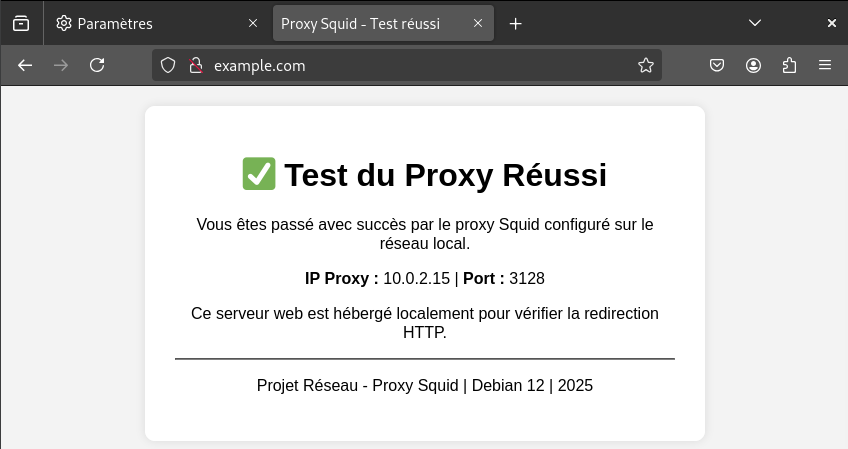
\includegraphics[width=1\linewidth]{img.png}
    
\end{figure}

\subsection{Analyse des logs}
Squid garde une trace des requêtes dans ses journaux :
\begin{lstlisting}[language=bash]
cat /var/log/squid/access.log
\end{lstlisting}
Les logs permettent de contrôler l'activité du proxy, analyser les requêtes filtrées ou autorisées.

\section{Conteneurisation avec Docker}
\subsection{Conteneurisation de l’installation de Squid sous Docker en créant un Dockerfile.}
Voici les étapes pour installer Docker sur Debian
\begin{lstlisting}[language=bash]
sudo apt update
sudo apt install -y docker.io
sudo systemctl enable docker
sudo systemctl start docker
\end{lstlisting}
Et on verifie si le Docker est bien installé et fonctionne normal avec cette commande :
\begin{lstlisting}[language=bash]
docker --version
\end{lstlisting}
Puis on crée un répertoire de travail squid-docker
\begin{lstlisting}[language=bash]
mkdir /etc/squid-docker 
cd \~/squid-docker 
\end{lstlisting}
Et puis on crée un fichier nommé squid.conf (pour Docker) qui contient la configuration de squid, dans ce même repertoire :
\begin{lstlisting}[language=bash]
nano squid.conf
\end{lstlisting}
Et on configure ce fichier par ce script (pour Docker) 
\begin{lstlisting}
http_port 3128
acl localnet src 0.0.0.0/0
http_access allow localnet
http_access deny all
visible_hostname squid-docker
\end{lstlisting}
\subsubsection{Création du Dockerfile}
On crée un fichier Dockerfile dans le même répertoire squid-docker.

Un Dockerfile contient les instructions suivantes pour construire l'image d'un conteneur. 
\begin{lstlisting}[language=bash]
nano Dockerfile 
\end{lstlisting}
Voici l’étape de création de ce fichier Dockerfile

\begin{lstlisting}
FROM debian:12
LABEL maintainer="TonNom <ton.email@example.com>"
LABEL description="Image Docker de Squid Proxy simple"
\# Installer Squid
RUN apt update \&& apt install -y squid \&& apt clean
\# Copier la configuration personnalisée
COPY squid.conf /etc/squid/squid.conf
\# Ouvrir le port du proxy
EXPOSE 3128
\# Lancer squid au démarrage du conteneur
CMD ["squid", "-N", "-d", "1"]

\end{lstlisting}

\subsubsection{Construction et exécution}
\begin{lstlisting}[language=bash]
cd /etc/squid-docker

docker build -t squid-proxy .
docker run -d --name squid-container -p 3128:3128 squid-proxy
\end{lstlisting}
\subsection{Test dans navigateur ou via curl}
Avant tout, il faut bien vérifier si le conteneur tourne ou non :

\begin{lstlisting}[language=bash]
docker ps
\end{lstlisting}
Et puis on fait un test dans le navigateur comme on a fait pendant le test du serveur proxy mais cette fois avec la conteneurisation :

\begin{itemize}
    \item On va dans les paramètres réseau → proxy manuel
\end{itemize}
\begin{itemize}
    \item Adresse : localhost
\end{itemize}
\begin{itemize}
    \item Port : 3128
\end{itemize}
\begin{itemize}
    \item Teste http://example.com
\end{itemize}

Pour autre vérification
\begin{lstlisting}[language=bash]
curl -x http://localhost:3128 http://example.com
\end{lstlisting}
Et après la page HTML s’affiche, ça veut dire que le proxy fonctionne bien
\subsection{Documentation sur les installations et l’utilisation de l’image Docker créé}
Pour permettre un déploiement rapide et portable via Docker, il nous faut une conteneurisation du Squid Proxy. Pour ce faire, on a besoin deux fichiers qui sont Dockerfile et squid.conf. Le fichier Docker contient : l’image de base qui est Debian 12, l’installation de Squid, copie d’une configuration minimale, exposition du port 3128.

Voici les étapes et les commandes utilisés pour le lancer, en résumé :
\begin{lstlisting}[language=bash]
\# Construire l’image
docker build -t squid-proxy .
\# Lancer le conteneur
docker run -d --name squid-container -p 3128:3128 squid-proxy
\# Vérifier si ça fonctionne
curl -x http://localhost:3128 http://example.com 
\end{lstlisting}
Et il est bien à noter que notre conteur fonctionne sans authentification et peut être adapté pour l’intégrer à un réseau interne.

\section*{Conclusion}
Ce mini-projet a permis d’explorer et de maîtriser plusieurs aspects fondamentaux de l’administration réseau et système, en s’appuyant sur un outil professionnel et libre qui est Squid. À travers les différentes étapes, l’installation sur une machine Debian, jusqu’à la création d’une image Docker fonctionnelle, nous avons mis en œuvre une solution efficace, portable et automatisée de proxy HTTP.

Les tests réalisés ont confirmé le bon fonctionnement du serveur, avec des règles d’accès configurées et des connexions filtrées selon des politiques précises. L’automatisation par script Bash facilite la reproductibilité de l’installation, et la conteneurisation via Docker assure une grande souplesse de déploiement, quelles que soient les plateformes.

Ce projet constitue une base solide pour des extensions futures telles que : l’intégration d’une authentification utilisateur, la mise en place d’un cache avancé, le filtrage par domaine, ou encore l’administration à distance via une interface Web.


\end{document}
